\documentclass[12pt]{beamer}
\usetheme{Penn} 
\usepackage{amsmath, amssymb, amsthm, amsfonts}
\usepackage{graphicx}
\usepackage{fancyvrb}
\usepackage{verbatim}
%\usepackage{tabularx}
\usepackage{tikz}
\usepackage{animate}
\usetikzlibrary{matrix, shapes, arrows, calc, backgrounds}
\usepackage[vcentermath, enableskew]{youngtab}
\newcommand{\ZZ}{\ensuremath{\mathbb{Z}}}
\newcommand{\RR}{\ensuremath{\mathbb{R}}}
\newcommand{\PP}{\ensuremath{\mathbb{P}}}

\newcommand{\CC}{\ensuremath{\mathbb{C}}}

\newtheorem{thm}{Theorem}[section]
\newtheorem{cor}[thm]{Corollary}
\newtheorem{lem}[thm]{Lemma}
\newtheorem{prop}[thm]{Proposition}
\theoremstyle{definition}
\newtheorem{conj}[thm]{Conjecture}
\newtheorem{defn}[thm]{Definition}
\newtheorem{ex}[thm]{Example}
\newtheorem{rmk}[thm]{Remark}
\newtheorem{alg}[thm]{Algorithm}
\newtheorem{question}[thm]{Question}
\begin{document}

\author[Z. Rosen]{Zvi Rosen \\ Department of Mathematics}

\date[\today]{\today}
\title[Matrices]{{\Large Linear Algebra}}
\institute[Dept. of Mathematics~~--~~University of Pennsylvania]{}


\frame{\titlepage}

\begin{frame}
\frametitle{Usual way we talk about matrices}

A real $m\times n$ matrix $A$ is a grid of numbers $A_{ij}$
with $i = 1,\ldots,m$ and $j = 1,\ldots,n$.
\vspace{2mm}

Matrix multiplication is an operation that takes two matrices
$A,B$ of dimensions $l\times m$ and $m\times n$ and returns a third matrix 
$C$ of dimensions $l \times n$ by the following rule:
\[ C_{ij} = \sum_{k = 1}^m A_{ik} B_{kj}
\]
\end{frame}

\begin{frame}
\frametitle{Matrices as linear maps}


A real $m\times n$ matrix $A$ is a function that
eats vectors in $\RR^n$ and spits out vectors in $\RR^m$.\\
\vspace{2mm}
The entry $A_{ij}$ is the number in the $j$-th coordinate of the
output when your input is the $i$-th unit vector.
\vspace{2mm}

Matrix multiplication takes two of these functions $A,B$, for which
$B$ eats vectors in $\RR^n$ and spits out vectors in $\RR^m$, and
$A$ eats vectors in $\RR^m$ and spits out vectors of $\RR^l$, and it
describes the function composition $C$ which acts by sending the
vector from $\RR^n$ through $B$ then $A$.
\end{frame}

\begin{frame}
\frametitle{Matrices as linear maps - Picture}
The following map from $\RR^2$ to $\RR^2$ rotates
and scales the basis vectors.

\centerline{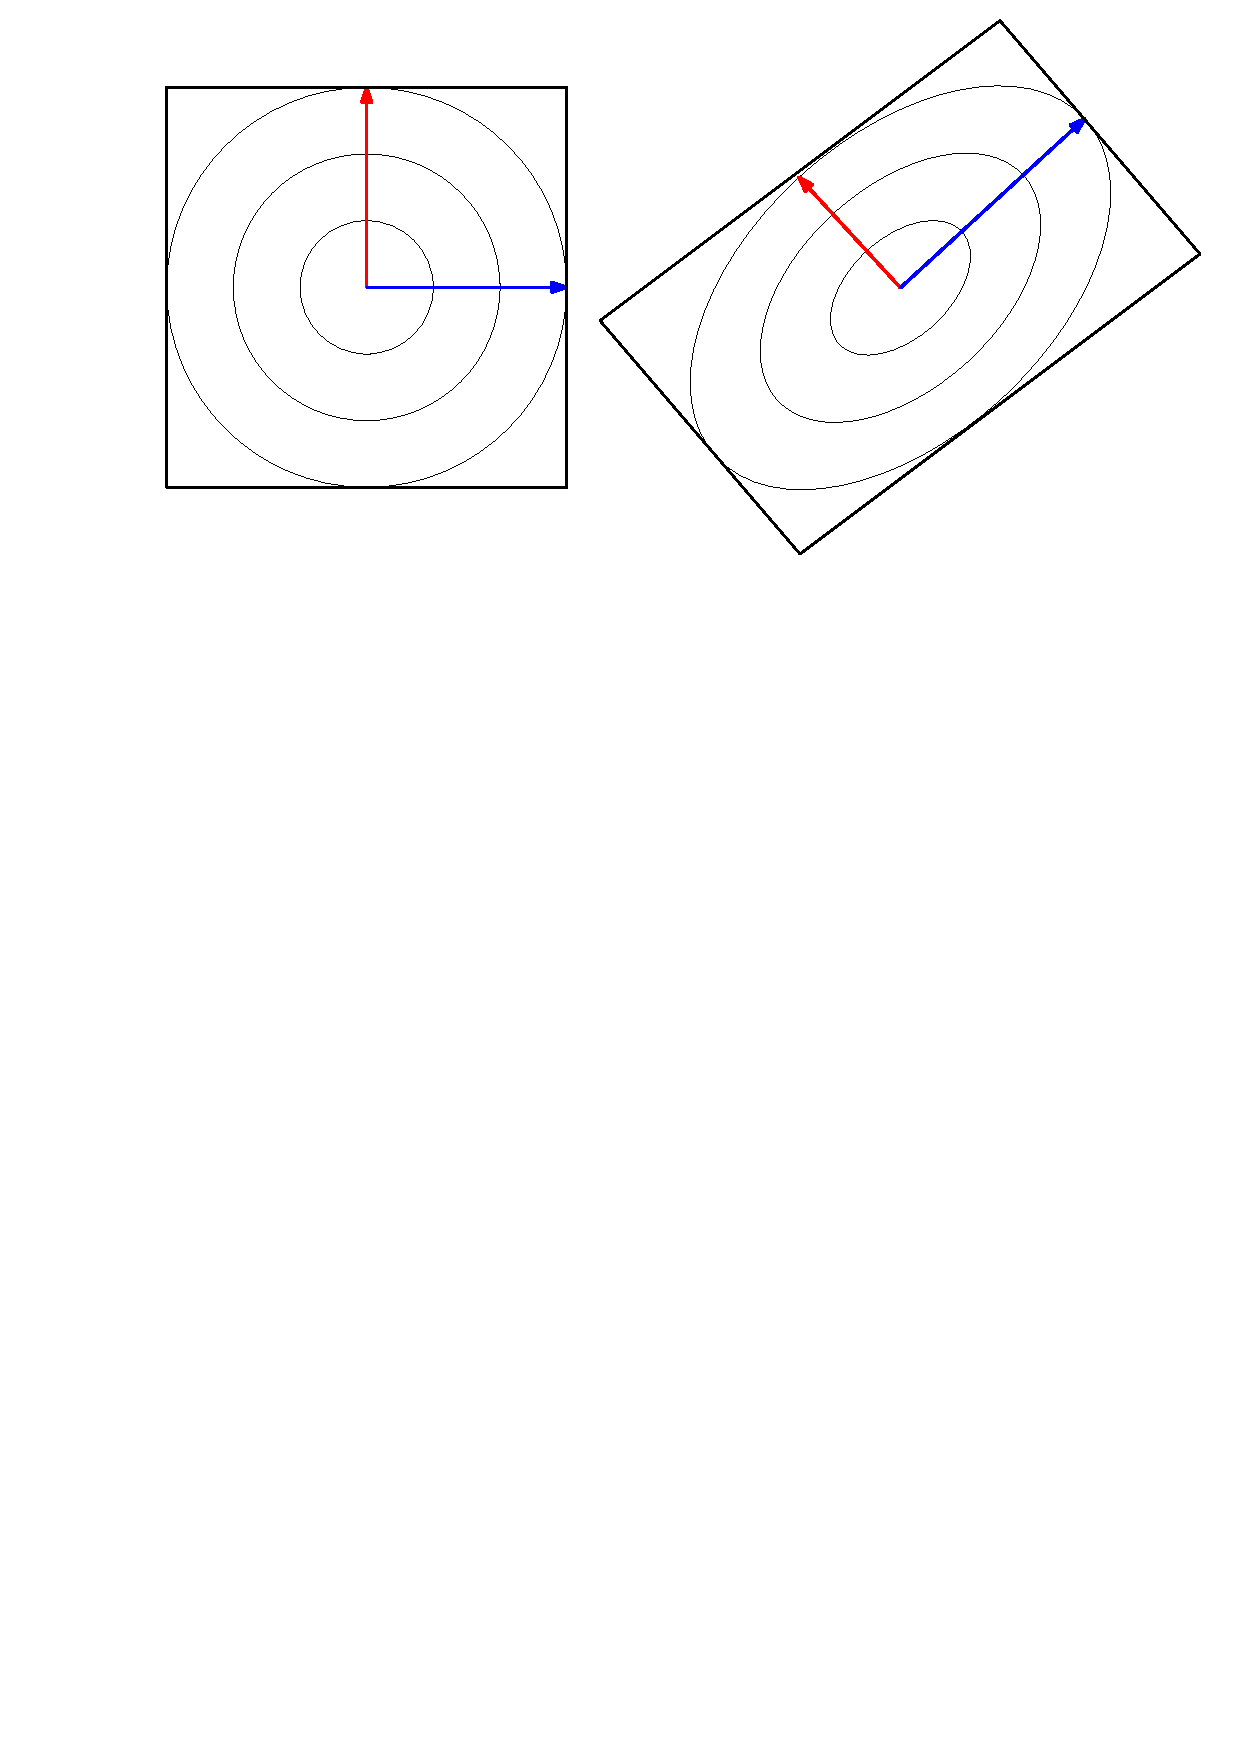
\includegraphics[width=.8\textwidth]{matr-pic.pdf}}

The corresponding matrix $A = \left( \begin{array}{cc}  1 & -1/2 \\ 1 & 1/2 \end{array} \right)$.
\end{frame}


\begin{frame}
\frametitle{Matrices as linear maps - Picture}
\centerline{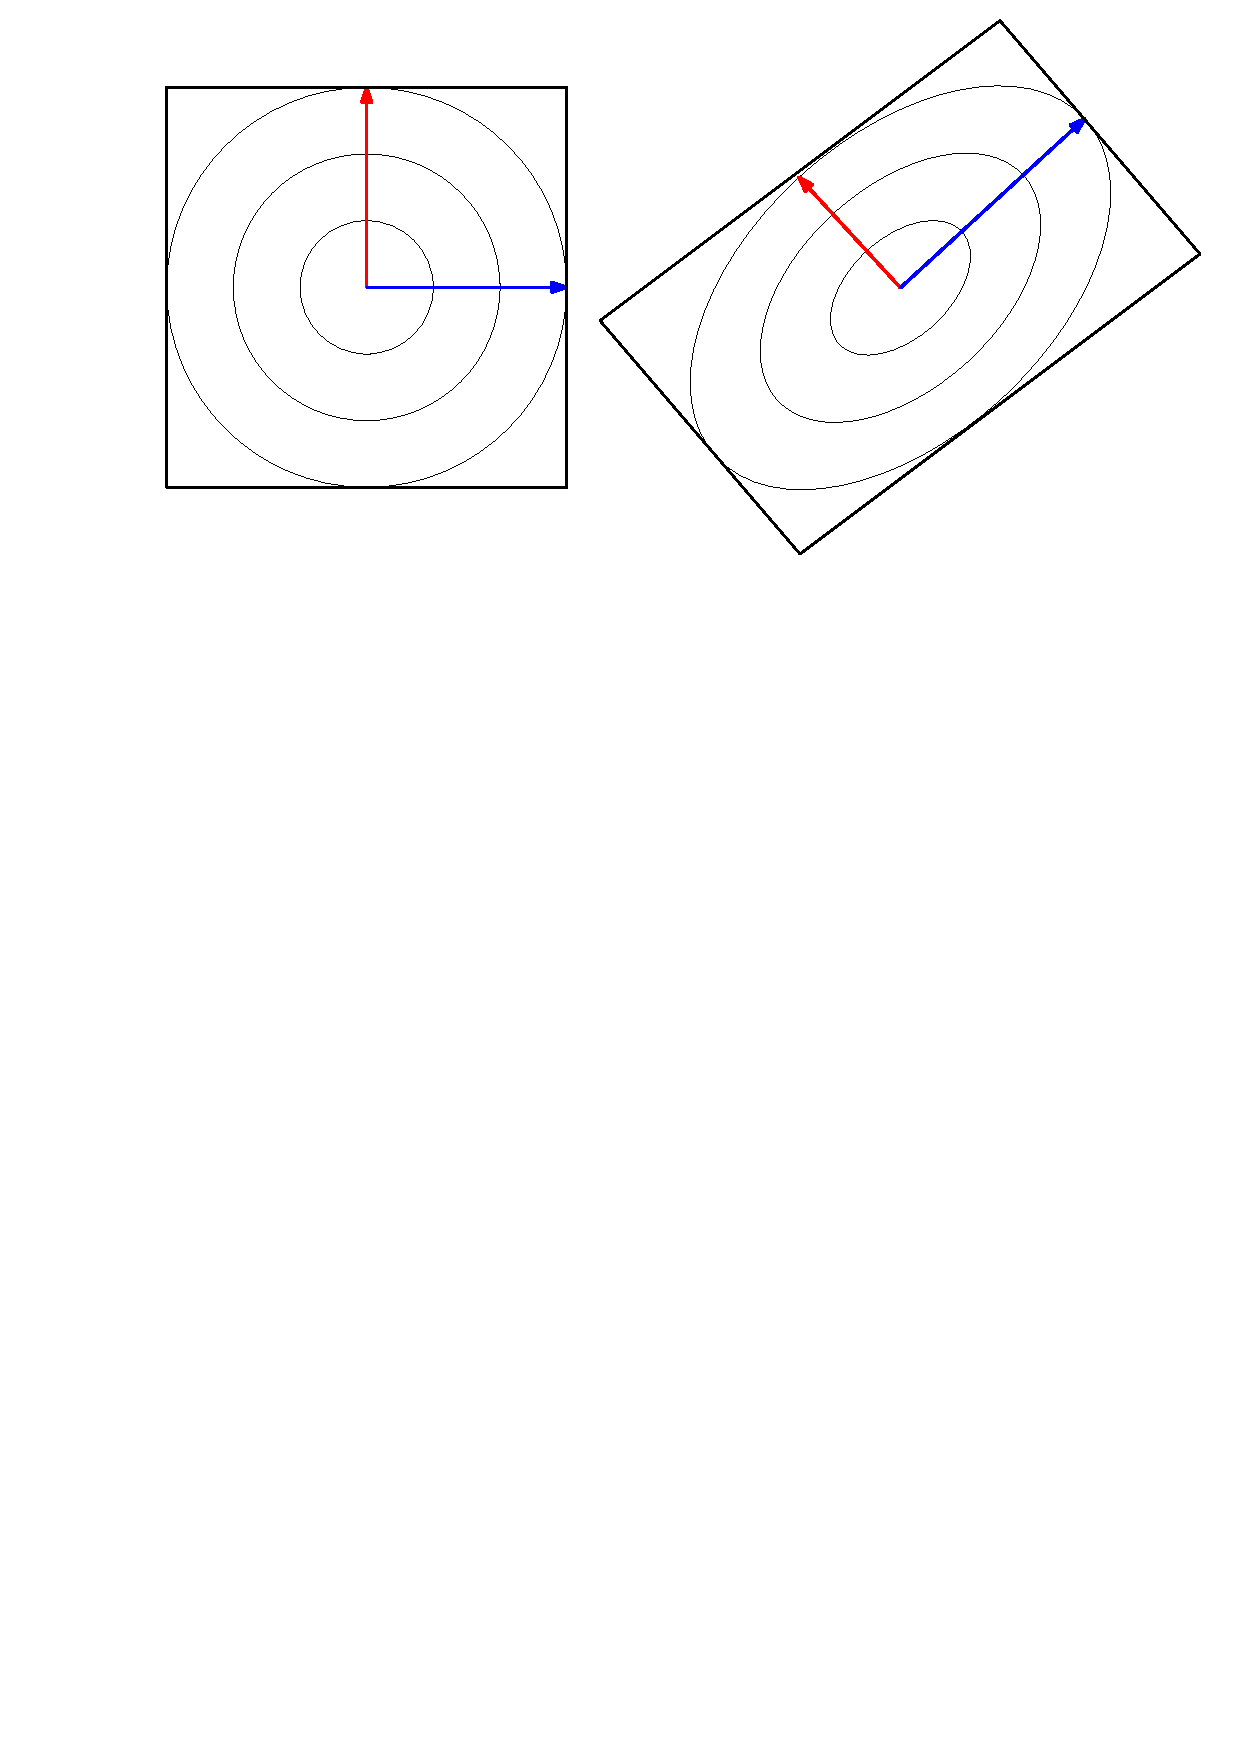
\includegraphics[width=.8\textwidth]{matr-pic.pdf}}

The corresponding matrix $A = \left( \begin{array}{cc} 1 & - 1/2  \\1 & 1/2 \\ \end{array} \right)$.\\
The first column tells us the output for input $(1,0)$,
and the second column gives the output for input $(0,1)$.
\end{frame}


\begin{frame}
\frametitle{Linearity}

A matrix defines a {\em linear map}. This means 
\[ A(c \vec{v} + d \vec{w}) = c \cdot A \vec{v} + d \cdot A \vec{w}.\]

In particular, scalar multiplication and addition of vectors
can be done before applying the function $A$ or after, and you'll
get the same result!
\end{frame}


\begin{frame}
\frametitle{Identity Matrix}
What matrix $I$ takes vectors in $\RR^n$ and
spits out the same vector?


\[ I  = \left( \begin{array}{ccccc}  
1 & 0 & \cdots & 0 \\
0 & \ddots &  & \vdots \\
\vdots &  & 1 & 0 \\ 
0 & \cdots & 0 & 1
\end{array} \right).\]

\end{frame}


\begin{frame}
\frametitle{Inverse Matrix}
If a matrix $A$ is a function eating vectors in $\RR^n$ and
spitting out vectors in $\RR^n$, the inverse matrix $A^{-1}$ eats
the output and spits out the input.
$A^{-1}  = \left( \begin{array}{cc}  1/2 & 1/2  \\-1 & 1 \\ \end{array} \right)$.

\centerline{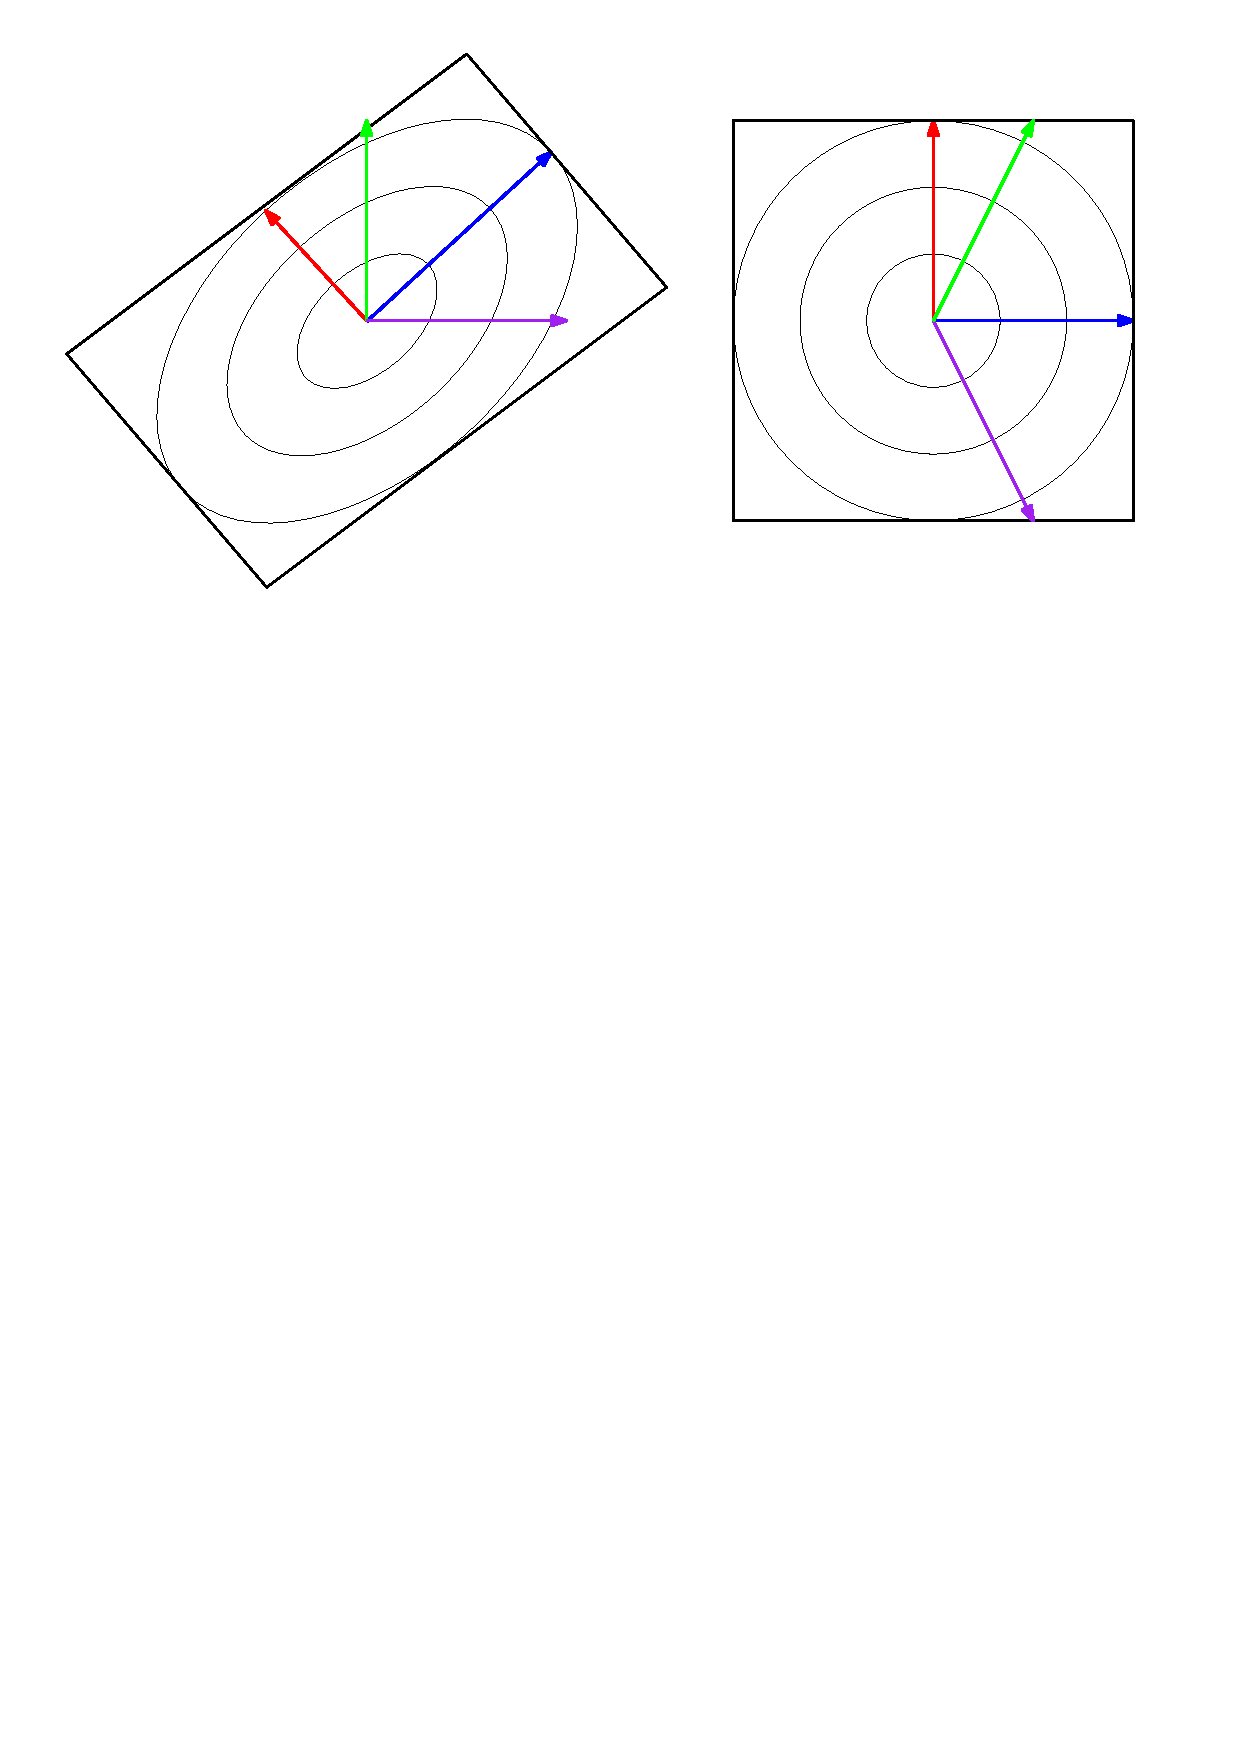
\includegraphics[width=.8\textwidth]{matr-pic2.pdf}}

\end{frame}

\begin{frame}
\frametitle{Inverse Sanity Check}
If $A$ is an $m \times n$ matrix instead of an $n \times n$ square matrix,
does the inverse exist?
\begin{itemize}
\item If $m > n$, the image of the smaller space does not fill up the larger space.
A matrix $\hat{A}$ which acts as an inverse on the image of $A$ exists, but it
is not unique.

\item If $n > m$, the larger space gets squashed into the smaller space, so many
vectors get mapped to the same vector.
\end{itemize}
\end{frame}


\begin{frame}
\frametitle{Not all square matrices are invertible}

A square matrix is invertible if and only if 
its {\em determinant} is nonzero. We will study determinants
in the next lecture. An example of a non-invertible matrix is:
\[
 \left(
\begin{array}{ccccccc}
1 & 2 & 3 \\
4 & 5 & 6 \\ 
1 & 1 & 1 \\ 
\end{array} \right) 
\]
In terms of the linear map, if the matrix is not invertible,
the map puts vectors into a smaller-dimensional space. For example,
the image of this matrix is 2-dimensional.

\end{frame}

\begin{frame}
\frametitle{Linear algebraic equations in Matrix Form}

The following is a linear system of equations, because
every terrm only has a single $x$ variable in degree 1:
\[
\begin{array}{ccccccc}
a_{11} x_1 & + & a_{12}x_2 &  + & a_{13} x_3 & = & b_1 \\
a_{21} x_1 & + & a_{22}x_2 &  + & a_{23} x_3 & = & b_2 \\
a_{31} x_1 & + & a_{32}x_2 &  + & a_{33} x_3 & = & b_3 \\
\end{array}
\]
It can be summarized as $A \vec{x} =\vec{b}$. 
\[ \left(
\begin{array}{ccccccc}
a_{11}  & a_{12} & a_{13} \\
a_{21}  & a_{22} & a_{23} \\ 
a_{31}  & a_{32} & a_{33} \\ 
\end{array} \right) \left( \begin{array}{c}
x_1 \\ x_2 \\ x_3 \end{array}
\right) =
 \left(
\begin{array}{ccccccc}
b_1\\
b_2 \\ 
b_3\\
\end{array} \right)
\]
\end{frame}


\begin{frame}
\frametitle{Linear algebraic equations in Matrix Form}

The system $A \vec{x} =\vec{b}$ can also be considered
in terms of $A$ as a function on vector spaces.
\vspace{3mm}

i.e. {\em What vector $\vec{x}$ gives $\vec{b}$ as the output
when you run it through $A$?}
\vspace{3mm}

If $A$ is an invertible square matrix, then you can just run $\vec{b}$
through $A^{-1}$ to find the desired $\vec{x}$.

\end{frame}

\begin{frame}[fragile]
\frametitle{Using MATLAB to define matrices}
The first matrix definition below explicitly lists entries. The 
others define special matrices. Try them on MATLAB.

\begin{verbatim}

A = [1,2;5,6];
B = zeros(3,4);
C = ones(2,3);
D = eye(5);
\end{verbatim}

\end{frame}


\begin{frame}[fragile]
\frametitle{Using MATLAB to solve linear systems}

Let $A$ be an $n\times n$ square matrix defining a
system of linear algebraic equations as $A \vec{x} = \vec{b}$.

\vspace{5mm}

The following commands in MATLAB solve for $x$.
\begin{verbatim}
x = A\b;
x = inv(A)*b;
\end{verbatim}

\end{frame}

\begin{frame}
\frametitle{Other matrix operations}
The following are also matrix operations in MATLAB, for 
$A, B$ both $m \times n$ matrices, and $c$ a scalar:
\begin{enumerate}
\item {\tt A + B}, coordinate-wise addition.
\item {\tt A .* B}, coordinate-wise multiplication.
\item {\tt c * A}, scalar multiplication by a matrix.
\item {\tt A'}, transpose of the matrix.
\end{enumerate}
\end{frame}

\end{document}
